\documentclass{article}
\usepackage{tikz}
\usetikzlibrary{patterns}
\usepackage{pgfplots}
\title{Lab Work 2}
\author{Shijagurumayum Nganaremba Sharma}

\begin{document}
\maketitle

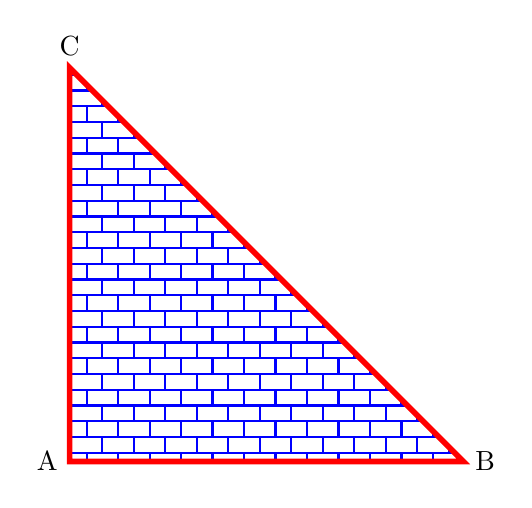
\begin{tikzpicture}
\pattern[pattern=bricks, pattern color= blue](0,0)--(0,5)--(5,0)--cycle;
\draw[line width=2pt, color=red](0,0)node[left, text=black]{A}--(0,5)node[above, text=black]{C}--(5,0)node[right,text=black]{B}--cycle;
\end{tikzpicture}

\vskip50pt

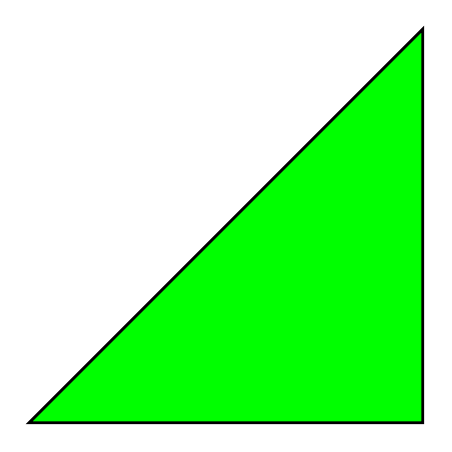
\begin{tikzpicture}
\fill[color=green](0,0)--(5,0)--(5,5)--cycle;
\draw[color=black, line width=1pt](0,0)--(5,0)--(5,5)--cycle;
\end{tikzpicture}


\begin{tikzpicture}
\fill[color=green](0,0)--(5,0)--(5,5)--cycle;
\end{tikzpicture}

\vskip50pt
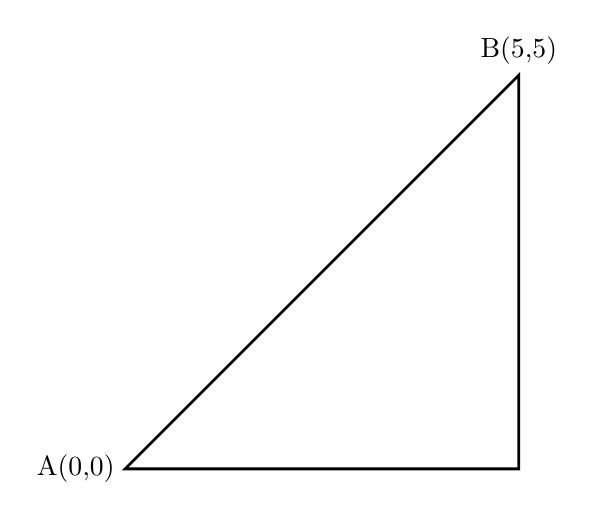
\begin{tikzpicture}
\draw[color=black, line width=1pt](0,0)node[left,color=black]{A(0,0)}--(5,0)--(5,5)node[above,color=black]{B(5,5)}--cycle;
\end{tikzpicture}

\vskip50pt

\begin{tikzpicture}
\shade[shading=ball, color=blue](0,0)rectangle(4,5);
\end{tikzpicture}

\vskip50pt
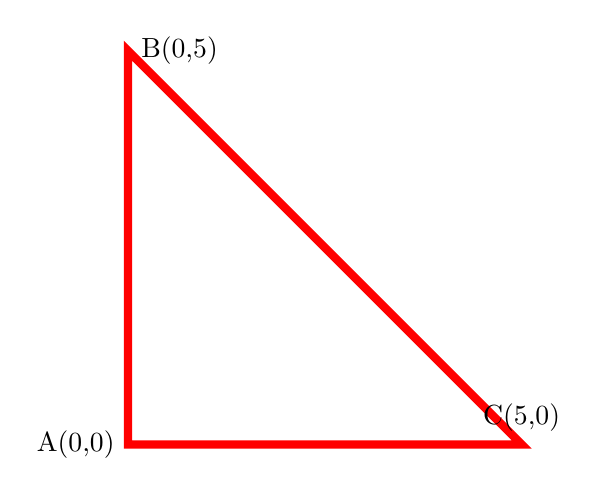
\begin{tikzpicture}
\draw[line width=3pt, color=red](0,0)node[text=black,left]{A(0,0)}--(0,5)node[text=black,right]{B(0,5)}--(5,0)node[text=black,above]{C(5,0)}--cycle;
\end{tikzpicture}

\vskip50pt
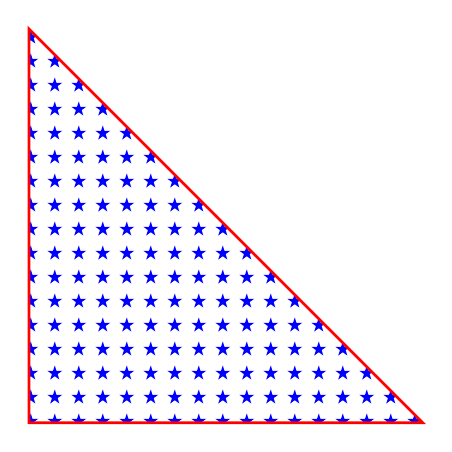
\begin{tikzpicture}
\pattern[pattern=fivepointed stars, pattern color=blue](0,0)--(0,5)--(5,0)--cycle;
\draw[line width=1pt, color=red](0,0)--(0,5)--(5,0)--cycle;
\end{tikzpicture}

\vskip50pt
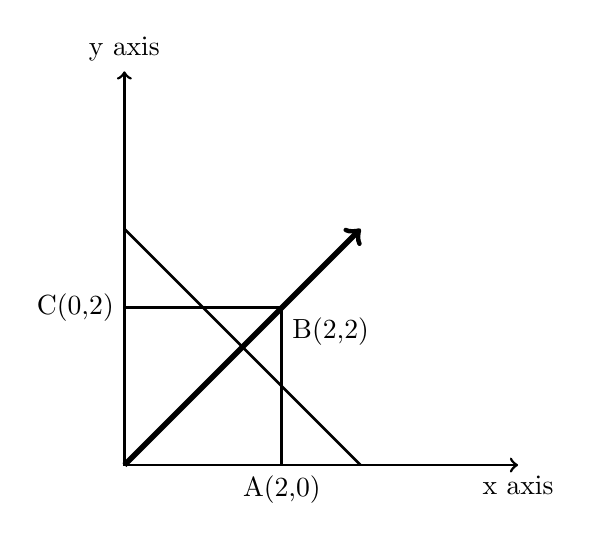
\begin{tikzpicture}
\draw[line width=1pt](0,0)--(0,2)node[left]{C(0,2)}--(2,2)node[below right]{B(2,2)}--(2,0)node[below]{A(2,0)}--cycle;
\draw[line width=1pt,->](0,0)--(5,0)node[below]{x axis};
\draw[line width=1pt,->](0,0)--(0,5)node[above]{y axis};
\draw[line width=1pt](0,3)--(3,0);
\draw[line width=2pt,->](0,0)--(3,3);
\end{tikzpicture}

\vskip50pt
\begin{tikzpicture}
\draw[line width=1pt](0,0)node[below left]{$A$}--(5,0)node[below right]{$B$}--(5,5)node[above right]{$C$}(0,0)--(0,5)node[above left]{$D$};
\draw[->,line width=1.5pt](5,5)--(0,5);
\end{tikzpicture}

\vskip50pt
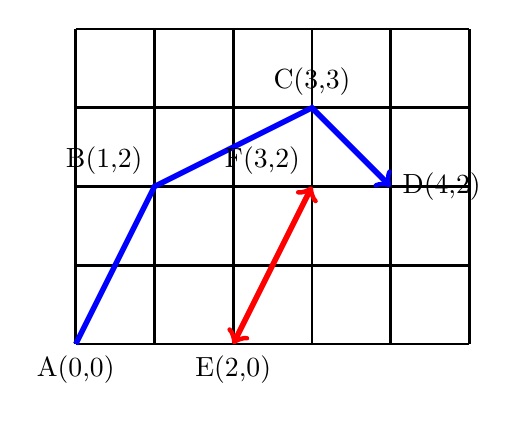
\begin{tikzpicture}
\draw[line width=1pt](0,0)grid(5,4);
\draw[line width=2pt,->,color=blue](0,0)node[below, color=black]{A(0,0)}--(1,2)node[above left, color=black]{B(1,2)}--(3,3)node[above, color=black]{C(3,3)}--(4,2)node[right, color=black]{D(4,2)};
\draw[<->,color=red, line width=2pt](2,0)node[below, color=black]{E(2,0)}--(3,2)node[above left, color=black]{F(3,2)};
\end{tikzpicture}

\vskip50pt
\begin{tikzpicture}
\begin{axis}[xmax=6, xmin=-6, ymax=160,ymin=-20,legend entries={$y=exp(x)$}]

\addplot [color=red]{exp(x)};
\end{axis}
\end{tikzpicture}

\vskip50pt
\begin{tikzpicture}
\begin{axis}
[xmax=4,xmin=-4, ymax=4, ymin=-4, axis x line=center, axis y line=center, xlabel={x axis label}, ylabel={y axis label}]
\end{axis}
\end{tikzpicture}

\vskip50pt
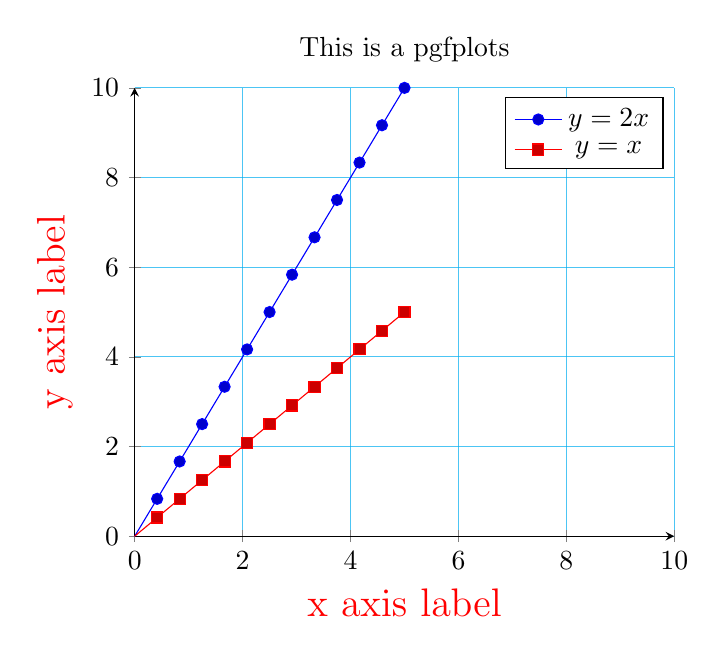
\begin{tikzpicture}
\begin{axis}
[ xmax=10, xmin=0, ymax=10, ymin=0, ylabel={\color{red}\Large y axis label}, xlabel={\color{red}\Large x axis label}, legend entries={$y=2x$,$y=x$}, title={This is a pgfplots},grid=major, grid style={cyan, opacity=0.7}, axis x line=bottom, axis y line = left]

\addplot{2*x};
\addplot{x};
\end{axis}
\end{tikzpicture}

\vskip50pt
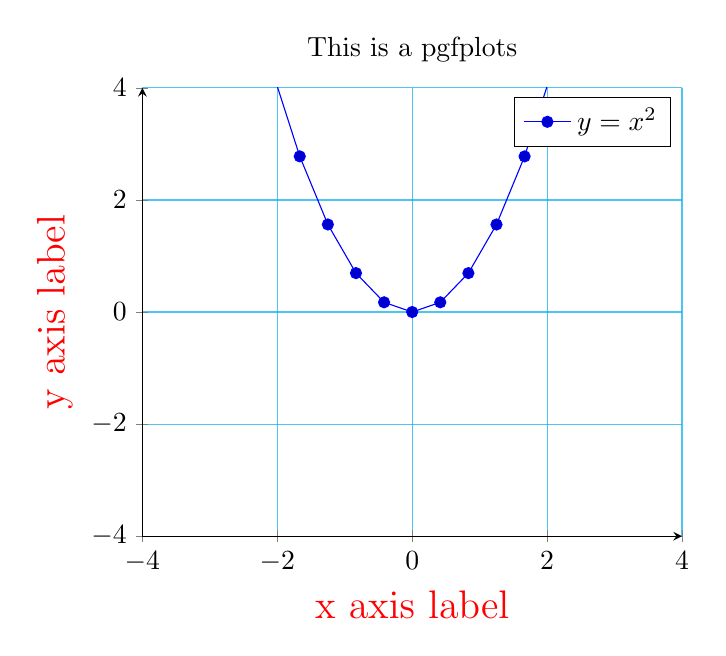
\begin{tikzpicture}
\begin{axis}
[ xmax=4, xmin=-4, ymax=4, ymin=-4, ylabel={\color{red}\Large y axis label}, xlabel={\color{red}\Large x axis label}, legend entries={$y=x^2$}, title={This is a pgfplots},grid=major, grid style={cyan, opacity=0.7}, axis x line=bottom, axis y line = left]

\addplot{x^2};
\end{axis}
\end{tikzpicture}

%%
\vskip50pt
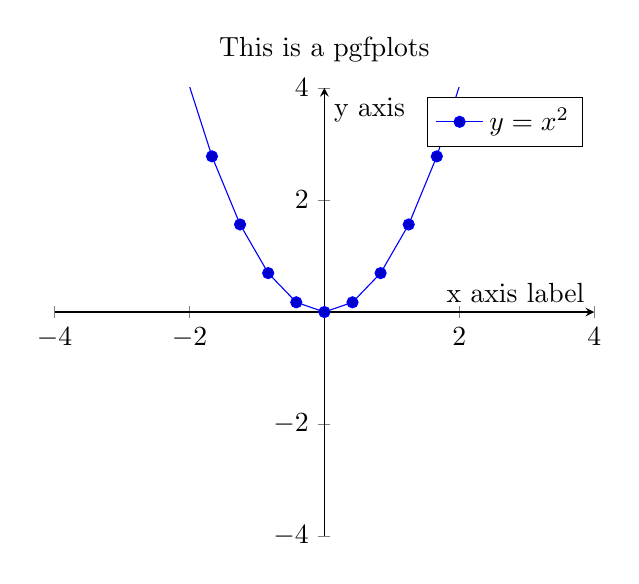
\begin{tikzpicture}
\begin{axis}
[xmax=4,xmin=-4,ymax=4,ymin=-4,legend entries={$y=x^2$}, xlabel={x axis label}, ylabel={y axis}, title={This is a pgfplots},axis x line=center, axis y line=center]

\addplot{x^2};
\end{axis}
\end{tikzpicture}

\vskip50pt
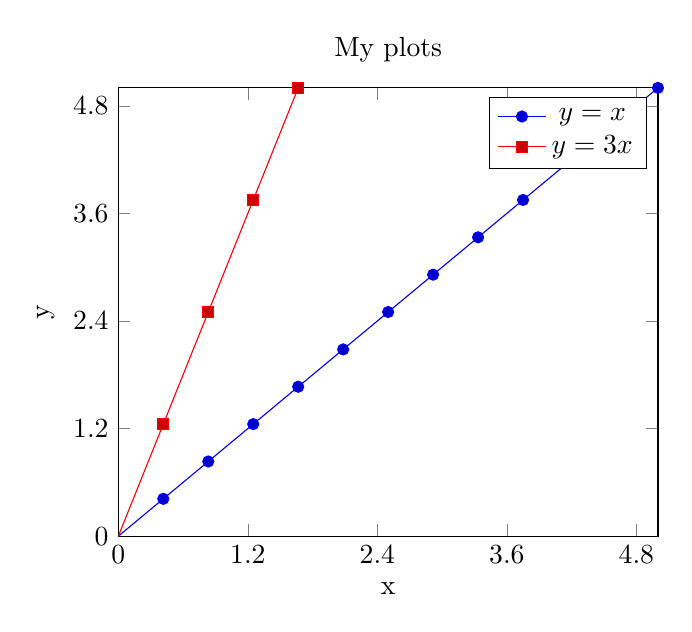
\begin{tikzpicture}
\begin{axis}
[xmax=5,xmin=0,ymin=0,ymax=5,legend entries={$y=x$,$y=3x$},xlabel={x},ylabel={y},xtick={0,1.2,...,5}, ytick={0,1.2,...,5}, title={My plots}]

\addplot{x};
\addplot{3*x};
\end{axis}
\end{tikzpicture}

\vskip50pt
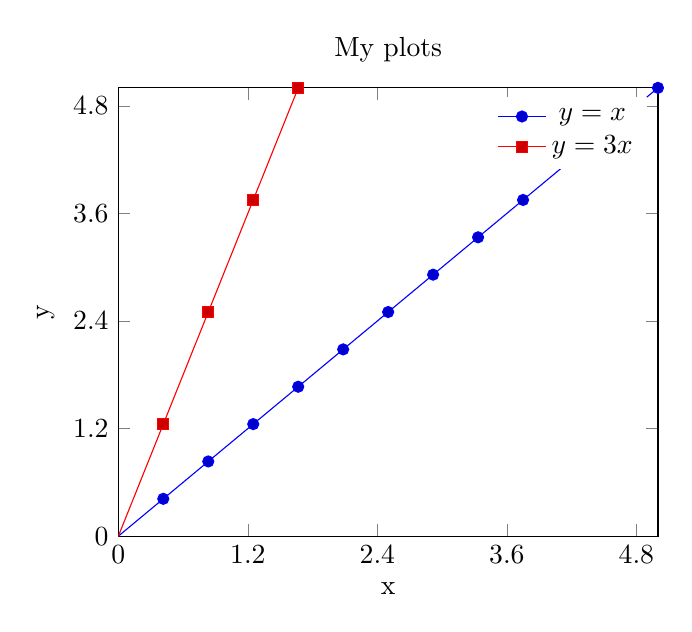
\begin{tikzpicture}
\begin{axis}
[xmax=5,xmin=0,ymin=0,ymax=5,legend entries={$y=x$,$y=3x$},xlabel={x},ylabel={y},xtick={0,1.2,...,5}, ytick={0,1.2,...,5},legend style={draw=none},title={My plots}]

\addplot{x};
\addplot{3*x};
\end{axis}
\end{tikzpicture}

\vskip50pt
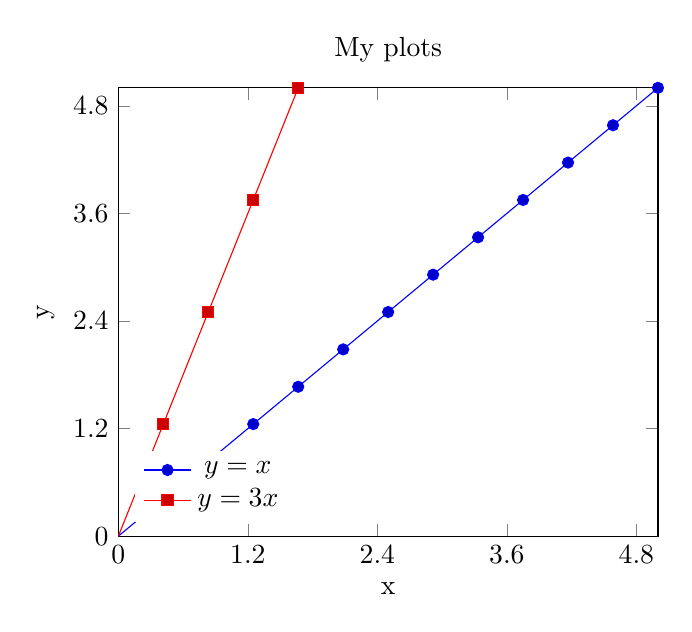
\begin{tikzpicture}
\begin{axis}
[xmax=5,xmin=0,ymin=0,ymax=5,legend entries={$y=x$,$y=3x$},xlabel={x},ylabel={y},xtick={0,1.2,...,5}, ytick={0,1.2,...,5},legend style={draw=none}, legend pos=south west,title={My plots}]

\addplot{x};
\addplot{3*x};
\end{axis}
\end{tikzpicture}

\vskip50pt
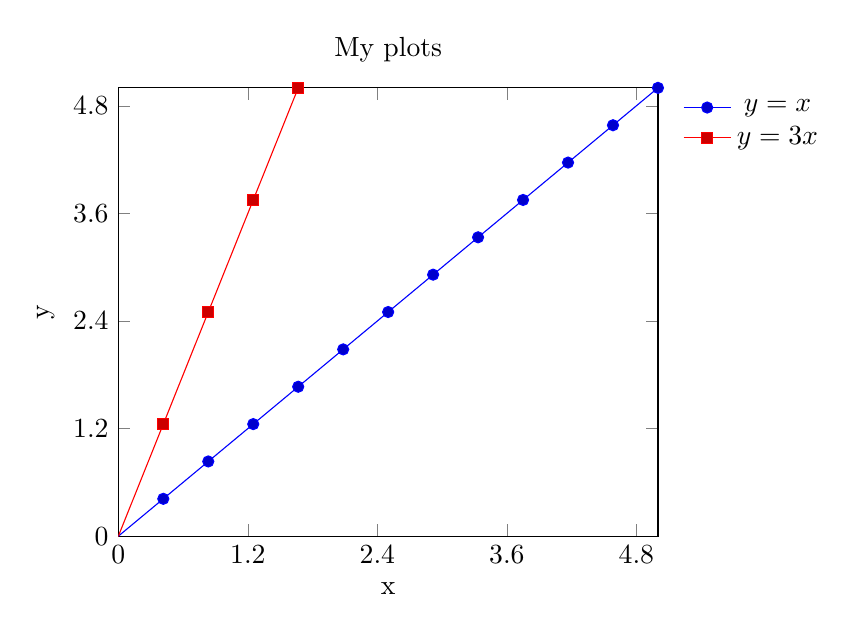
\begin{tikzpicture}
\begin{axis}
[xmax=5,xmin=0,ymin=0,ymax=5,legend entries={$y=x$,$y=3x$},xlabel={x},ylabel={y},xtick={0,1.2,...,5}, ytick={0,1.2,...,5},legend style={draw=none}, legend pos=outer north east,title={My plots}]

\addplot{x};
\addplot{3*x};
\end{axis}
\end{tikzpicture}

\vskip50pt
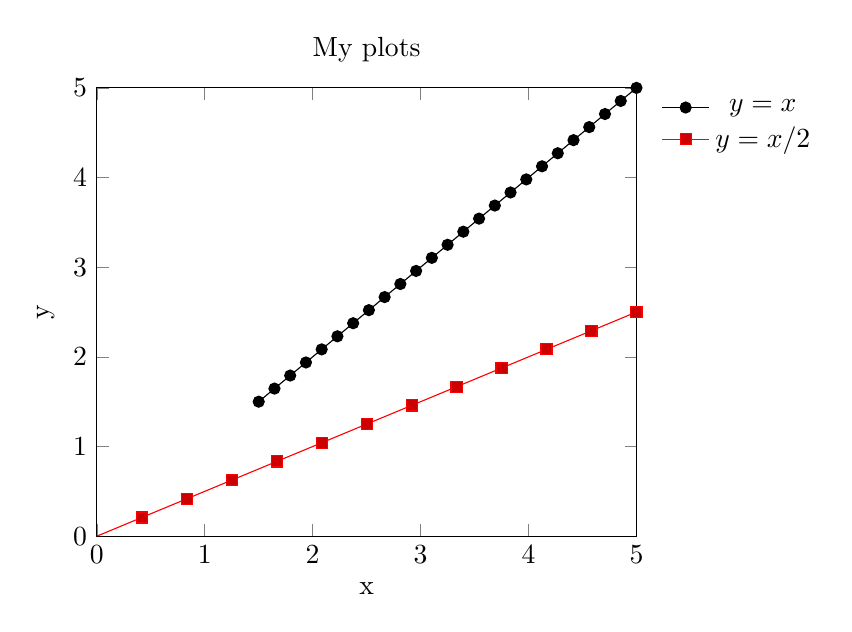
\begin{tikzpicture}
\begin{axis}
[xmax=5,xmin=0,ymin=0,ymax=5,legend entries={$y=x$,$y=x/2$},xlabel={x},ylabel={y},legend style={draw=none}, legend pos=outer north east,title={My plots}]

\addplot[color=black, mark=*, domain={1.5:5}]{x};
\addplot{x/2};
\end{axis}
\end{tikzpicture}

\vskip50pt
\begin{tikzpicture}
\begin{axis}
[xmax=5,xmin=0,ymin=0,ymax=5,legend entries={$y=x$,$y=x/2$},xlabel={x},ylabel={y},legend style={draw=none}, legend pos=outer north east,title={My plots}]

\addplot[color=black, mark=*, domain={1.5:4.5}, samples=10]{x};
\addplot[mark=+, color=red, samples=38]{x/2};
\end{axis}
\end{tikzpicture}

\vskip50pt
\begin{tikzpicture}
\begin{axis}
[xmax=5,xmin=0,ymin=0,ymax=5,legend entries={$y=x$,$y=x/2$},xlabel={x},ylabel={y},legend style={draw=none}, legend pos=outer north east,title={My plots}]

\addplot[color=black, mark=*, domain={1.5:4.5}, samples=10, draw=none]{x};
\addplot[mark=+, color=red, draw=none, samples=38]{x/2};
\end{axis}
\end{tikzpicture}

\vskip50pt
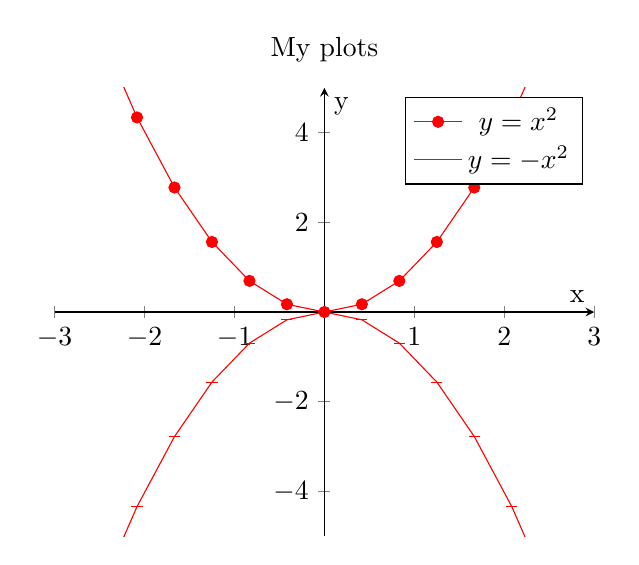
\begin{tikzpicture}
\begin{axis}
[xmax=3, xmin=-3, ymax=5, ymin=-5, axis x line=center, axis y line=center, legend entries={$y=x^2$,$y=-x^2$}, xlabel={x}, ylabel={y}, title={My plots}]
\addplot [mark=*, color=red]{x^2};
\addplot[color=red, mark=-]{-x^2};
\end{axis}
\end{tikzpicture}

\vskip50pt
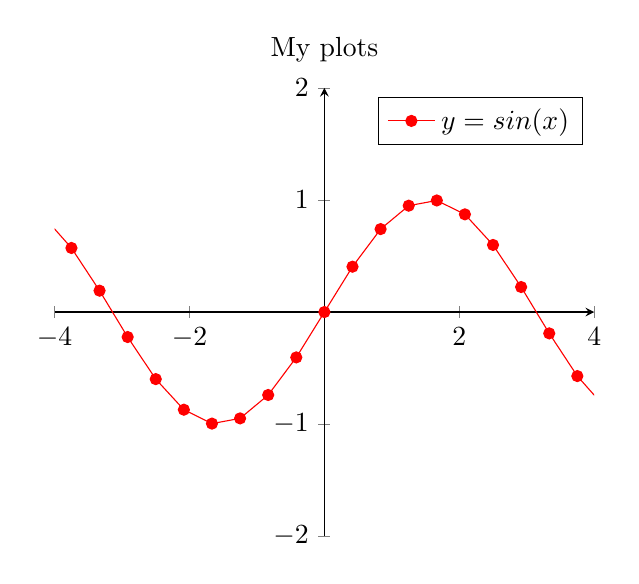
\begin{tikzpicture}
\begin{axis}
[xmax=4, xmin=-4, ymax=2, ymin=-2, title={My plots}, legend entries={$y=sin(x)$},axis x line=center, axis y line=center]

\addplot[color=red, mark=*]{sin(deg(x))};
\end{axis}
\end{tikzpicture}

\vskip50pt
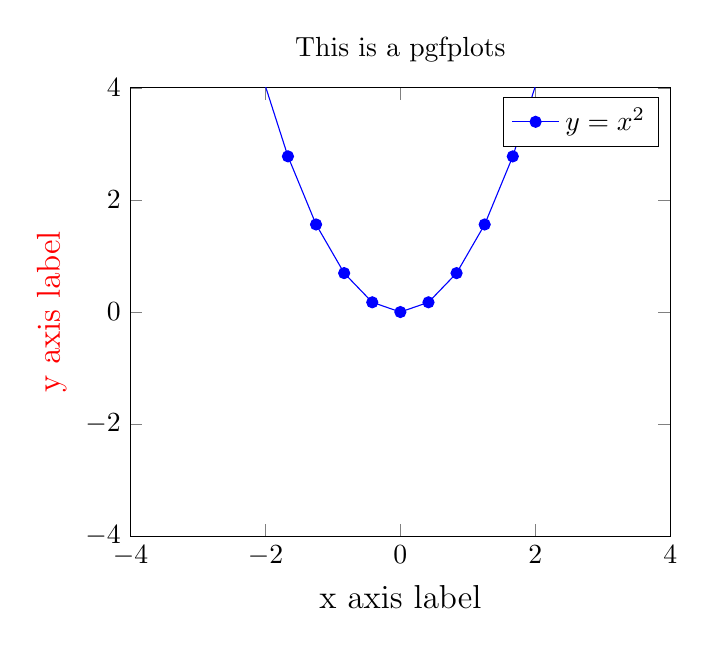
\begin{tikzpicture}
\begin{axis}
[xmax=4, xmin=-4, ymin=-4, ymax=4, title={This is a pgfplots}, xlabel={\large x axis label}, ylabel={\large \color{red} y axis label}, legend entries={$y=x^2$}]
\addplot[color=blue, mark=*]{x^2};
\end{axis}
\end{tikzpicture}

\vskip50pt
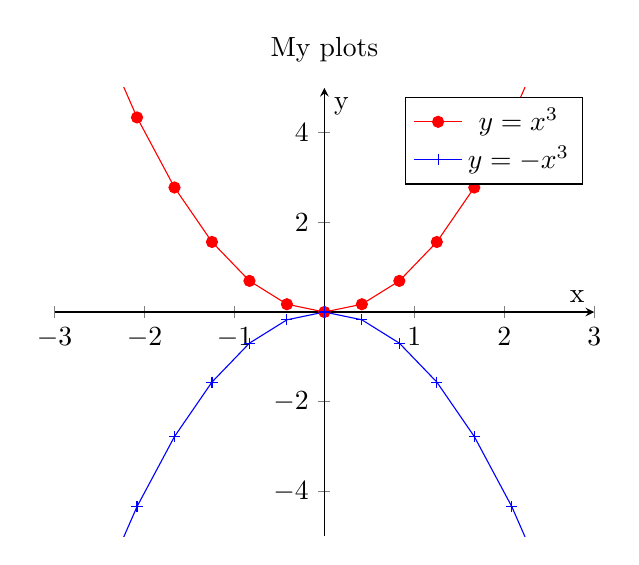
\begin{tikzpicture}
\begin{axis}
[xmax=3, xmin=-3,ymin=-5, ymax=5, xlabel={x}, ylabel={y}, title={My plots}, legend entries={$y=x^3$,$y=-x^3$}, axis x line=center, axis y line=center]
\addplot[color=red, mark=*]{x^2};
\addplot[color=blue, mark=+]{-x^2};
\end{axis}
\end{tikzpicture}

\end{document}
